\documentclass{llncs}

\usepackage[utf8]{inputenc}
\usepackage{url}
\usepackage{graphicx}
\graphicspath{{./images/}}

\title{Using hybrid human-machine workflows in creating original open Geographic Information}

\author{AUTHOR 1\inst{1}, AUTHOR 2\inst{1} \and AUTHOR 3\inst{2}}
\institute{INSTITUTE 1 \and INSTITUTE 2}

\date{December 2015}

\begin{document}

\maketitle

\begin{abstract}
As more open data is published by governments and organisations, the task of creating new open data changes from being a ground-up process - where data is collected and shaped from scratch - to an enhancement process, where pre-existing data sources, computation and original contributions by human participants - e.g. through crowdsourcing - are integrated together and enable each other through hybrid human-machine workflows. In this paper we present a possible application of such processes to a real world use case: the creation of "OLAF", an open address file for the UK. Experimental evaluation show the effectiveness of the approach.
\end{abstract}

\begin{keywords}
Crowdsourcing, Geographic Information, hybrid human-machine systems, open data 
\end{keywords}

[MAX 18 PAGES]

\section{Introduction}

\subsection{Crowdsourcing}

    Crowdsourcing is {[}...{]}. More generally {[}SOME LIGHTWEIGHT REFERENCE TO WHAT A SOCIAL MACHINE IS{]} [{[}BLAH BLAH SOCIAL MACHINES AS POSSIBLY ONE OF THE ONLY WAYS TO SOLVE PROBLEMS LIKE THIS + SOME EXCUSE TO CITE \cite{OReilly:2015uo}{]}

\subsection{Crowdsourcing Geographic Information}

    Among the many applications of crowdsourcing is the collection and maintenance of geospatial data, or "Geographic Information" (GI).
    
    Although it is commonly recognised for GI to have a significant economic and social value \cite{Sui:2012uf}[THIS IS A REFERENCE TO AN ENTIRE BOOK, LIKELY UNSUITABLE], the effort national mapping and cadastre agencies (NMCAs) worldwide put into producing and updating cartography has been in decline for several decades \cite{ESTES:1994vz}. In the U.S., for example, the Geological Survey (USGS) no longer attempts to update its maps on a regular basis and the National Research Council promotes a vision in which {[}...{]} \cite{Committee:1993vp}.
    
    {[}Somewhere in the literature someone said that the emergence of VGI was actually suggested by one of those authorities{]}
    
    Crowdsourcing GI is then seen as the cost effective and "good enough" solution to this problem [CITATION OF SOME SCHOLAR SAYING THAT GOOD ENOUGH IS... GOOD ENOUGH]. The phenomenon of {\it Volunteered} Geographic Information (VGI) in particular was studied extensively since the term was coined \cite{Goodchild:2007vt}. Developing understanding of VGI was made possible by the success of services such as Wikimapia\footnote{\url{http://wikimapia.org/}.} or OpenStreetMap\footnote{\url{http://www.openstreetmap.org/}.}. The latter is likely the best known VGI-based mapping service available today.

\subsection{Open data and open Geographic Information}

    Open data is data that anyone can access, use and share\footnote{\url{http://theodi.org/faq}.}. 
    
    NMCAs, as governments and private organisations, are becoming more sensitive to the opportunities arising from publishing and re-using open data. In Great Britain, for example, since 2015 the local NMCA Ordnance Survey\footnote{\url{http://www.ordnancesurvey.co.uk/}.} has released in the open a substantial volume of data that was previously available to the public as commercial products only, e.g. "Open Names"\footnote{\url{https://www.ordnancesurvey.co.uk/business-and-government/products/os-open-names.html}.}, a place-name index, and "Open Roads"\footnote{\url{https://www.ordnancesurvey.co.uk/business-and-government/products/os-open-roads.html}.}, the generalised geometry and network connectivity of the road network.
    
    The availability of such high quality and authoritative sources becomes a substantial enabler for the creation of new, original geospatial data. There where GI could only be created from scratch - as in OpenStreetMap's case when it was started in the UK in 2007 - it is now possible to rather focus the effort of the crowd on complementing what is already available, or augmenting it.

\subsection{Crowdsourcing open data}

    The work described in this paper took place in the context of a larger research programme aimed at assessing the feasibility of building original open data by using non-expert human contributions, technology systems and, where available, other pre-existing open data. 
    
    Although most of the effort of producing and releasing open data is commonly expected of governments and businesses, there are industry sectors and domains of knowledge where resistance to change can halt or substantially slow down this process. Demand and offer for open data is strongly suppressed, for example, due to failure in recognising open data-enabled business models, restrictive legislative and patent systems, or charging for public datasets \cite{shadboltpaf}. 
    
    The assumption at the base of our research is that the people's contribution is necessary to address this problem. People can be enabled, through technology, to capture and curate data, alongside what is already published by governments and businesses. Crowdsourcing is just one of the formulae by which socio-technical systems can be built for this purpose. This contribution is instrumental to delivering and curating the open data needed to build and operate a comprehensive {\it national information infrastructure} (NII).

\subsection{Challenges of crowdsourcing geospatial data}

    Two groups of challenges are relevant to the availability of good quality geospatial open data: on one side, exploiting it to improve the quality and enhance the functionality of pre-existing VGI initiatives, and, on the other, unleash completely new products and services.
    
    [CHALLENGE OF MAINTENANCE, AFTER COLLECTION]
    
    [SHOULD I WRITE MORE ABOUT THE OTHER CHALLENGES, TOO?]
    
    Completeness is a key element in the quality of geospatial data. In this paper we propose a method to improve the coverage of existing geospatial data where - for any reason - it is not possible to get volunteers to survey one specific geographical area or provide more detail than what is available already. This was described, for example, by **** , observing how OpenStreetMap volunteers naturally tend to avoid ***.
    
    {[}
    Add
    \begin{itemize}
    	\item {[}rationale of why we thought this was relevant, some justification in literature review{]}
    	\item {[}novelty of what we propose{]}
    \end{itemize}
    {]}
    
    {(}...{)}

\subsection{The Open Legal Address File}

    The main use case for this research is the attempt of creating a new geospatial dataset that is functionally equivalent to the "Postcode Address File" or "PAF"\footnote{PAF is a registered trademark by Royal Mail plc. For convenience we won't show the registered trademark sign "\textregistered" in this document every time we refer to it.}: a commercial dataset listing all known valid addresses and postcodes for the UK at a given point in time. 
    An act of law\footnote{The Postal Service Act 2000, part VII, article 116 \cite{postalserviceact2000}.} makes PAF ownership of the Royal Mail: the ex-postal service monopolist in the UK, now a public limited company with only a 30\% of shares controlled by the Government\footnote{The Postal Services Act 2011 plans to reduce the Government control down to 10\% \cite{postalserviceact2011}.}. The same act of law requires Royal Mail to make PAF available on "reasonable terms" to "any person who wishes to use it".
    
    To this day, though, the "reasonable terms" translated only into PAF being made available by Royal Mail and its resellers as a commercial product\footnote{As an end user who wants to access PAF's data one may incur Royal Mail licence fees going from \pounds0.012 per transaction on a public website to \pounds90,000 per year for unlimited internal use by a corporate group. Even charitable organisation may not take advantage of free PAF access unless their income is less than \pounds10m/year.}. This is considered an anomaly by many, as "reasonable terms for the external use of PAF data by third parties should be no more than the marginal cost of distribution (...)" \cite{odugresponse}. 

    To further limit the opportunities for PAF to be made open, in October 2013 Royal Mail and its assets were privatised, including PAF\footnote{\url{http://www.theguardian.com/uk-news/2014/mar/17/royal-mail-privatisation-ministers-rebuked-selling-data}}. The UK Parliament House of Commons' Public Administration Select Committee, just a few month later, called this "unacceptable and unnecessary" and recognised that PAF's "disposal for a short-term gain will impede economic innovation and growth" \cite{pascod}.

    This makes the opportunity of creating an alternative to PAF an ideal case study. We will call this the "Open Legal Address File", or "OLAF". The term "legal addresses" refers to all addresses that are, by law, in the public domain, hence have no restrictions in terms of intellectual property or privacy protection and can be published as open data\footnote{Legal addresses belong to either or both of the following two categories: a) they are the addresses of current or past UK residents who are or were registered on the public electoral register, and b) they are the addresses of past or present UK companies that are or were registered at the relevant British registrar, such as Companies House for England and Wales.}.

    {[}Definition of address{]}
    
    Many complementary and/or alternative strategies are possible and need to be used jointly to build OLAF. Among these is the opportunity to re-use published open datasets of addresses so to infer the existence of more addresses. 
    
    E.g. it is intuitive that if some source refers to the existence of house numbers 3, 5 and 9 in some street, and all are associated to the same postcode, it is very likely that number 7 exists as well and is associated to the same postcode\footnote{House numbering and postcode association are heavily dependant of the conventions used in the country the problem is applied to. This paper always refers to the UK conventions.}. It is shown experimentally that the method is effective, as it can produce large volumes of addresses from available open data\footnote{This was tested against the single largest known source of addresses open data for England and Wales: Land Registry's "Price Paid Data". See \url{https://www.gov.uk/government/collections/price-paid-data}.}.
    
    The experiments described in this paper implement the above strategy only, and  use crowdsourcing to validate sets of inferred addresses, as participants are asked to virtually survey the streets using pictures sourced from Google Street View.
    
    It has to be noted that not all existing house numbers are visible by surveying a street. E.g. there are no obligations in the UK to affix a house number or house name sign. Moreover, some of the house numbers may be associated to dwellings that are not visible unless the property is accessed, beyond what Google Street View's photos can capture.
    
    {(}...{)}
\section{Approach}

\subsection{The social machine mix}

    Although the OLAF data is conceptually simple, assembling such a large dataset as OLAF while assuring sufficient quality still is a complex task.
    
    It is our hypothesis that, to make the best use of pre-existing open data and potentially available technology and human resources, such a problem must be decomposed in a series of complementary sub-problems, each developing parts of its scope and leveraging the peculiarity of its specifications. Each problem, then, can be solved by designing a dedicated socio-technical system, or social machine. This decomposition can take place over several iterations, hence creating a hierarchy of systems that we will call the "social machine mix". 
    
    [THERE SHOULD BE AN IMAGE HERE BUT IMAGE POSITIONING IN LATEX IS TRICKY]

    \begin{figure*}
    	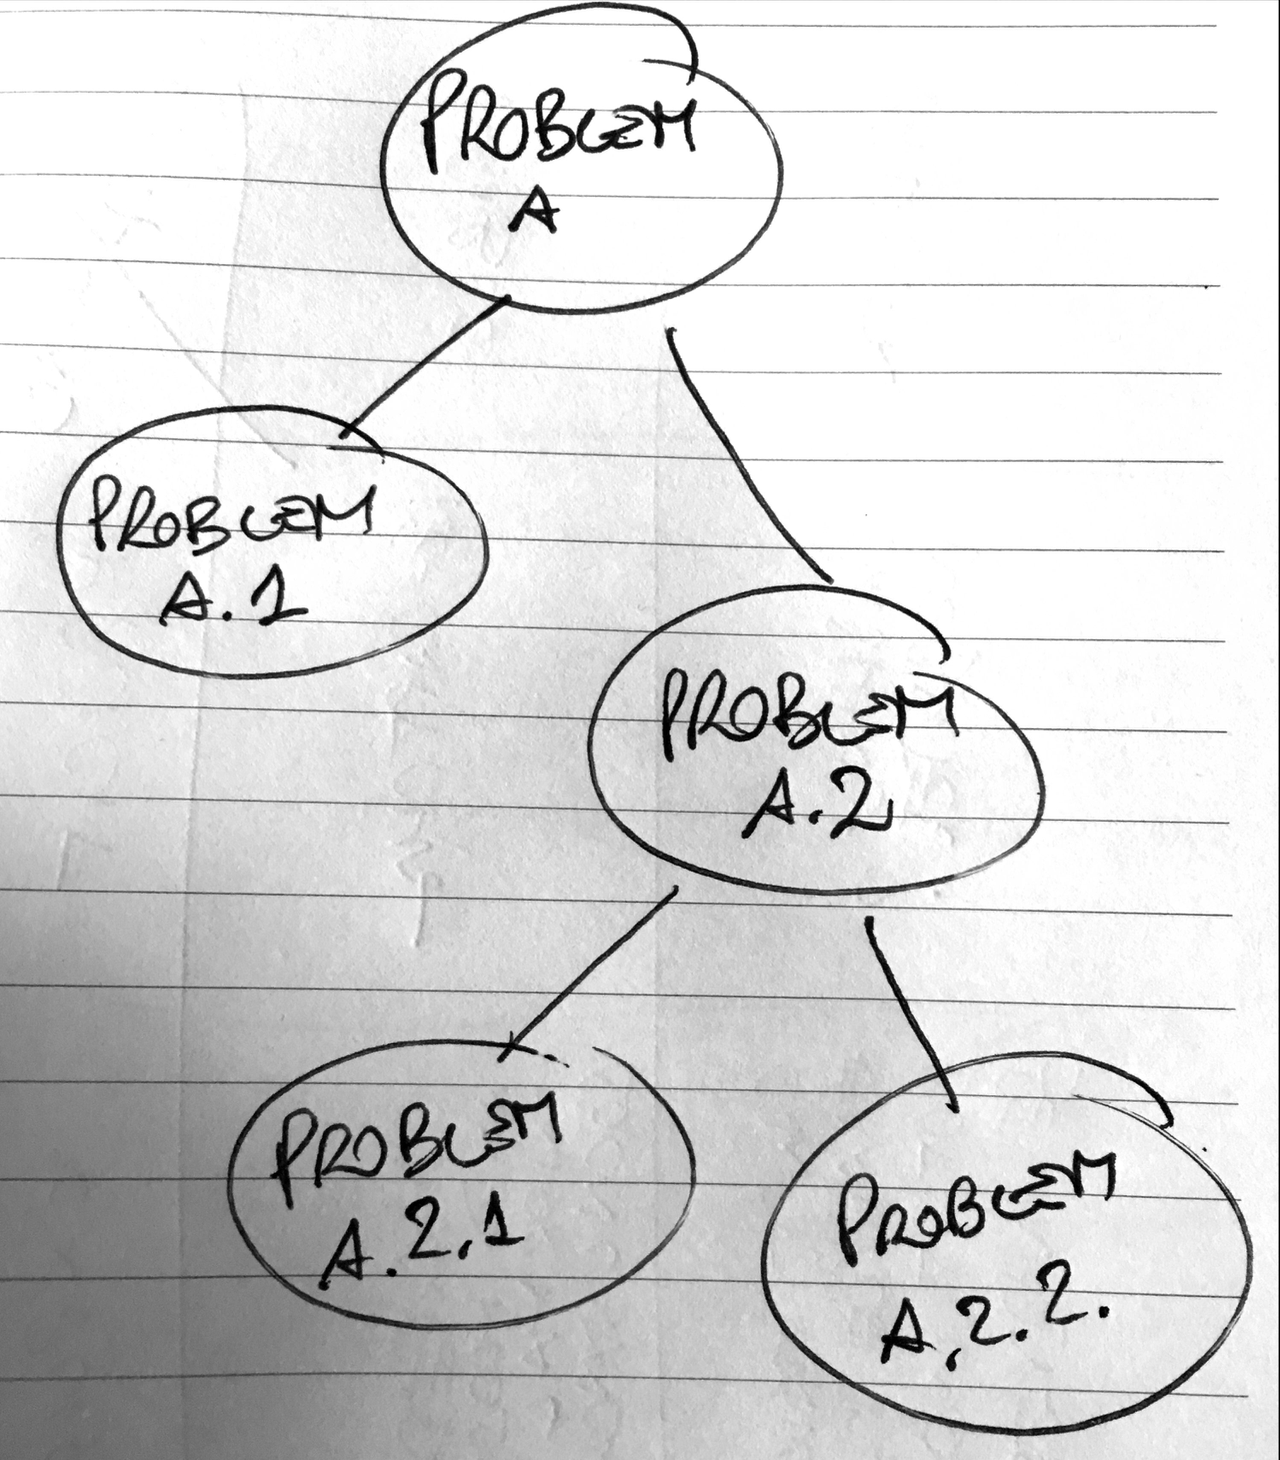
\includegraphics[width=0.95\textwidth]{social-machine-mix-1.png}
    	\caption{This picture should not be here, but apparently it is a nightmare in LaTeX.}
    	\label{fig:social_machine_mix_1}
    \end{figure*}
    
    \textbf{The central role of pre-existing open data.} 
    
    [THIS IS AN INTERESTING STATEMENT, I WONDER IF IT CAN BE GENERALISED] The main driver determining the possible decompositions of the original problem into a hierarchy of sub-problems is the availability of pre-existing and reliable open data. There are two reasons for that.

    \begin{itemize}

        \item The first and more intuitive reason is an assumption: no social machine can produce data in a more cost-effective way than re-using a pre-published, reliable dataset is.  
        
        Hence, the focus of social machines in the overall mix can only be of two kinds: a) on creating original data where the same cannot be sourced in any other machine-only method, and b) on leveraging those skills where humans outperform machines. The obvious example of this is the survey of the streets, being it in person in the physical world, or by examining pictures of the locations, that is how crowdsourcing is used in the system described later in this paper.

        \item The second reason is that open data can be instrumental to operate a social machine. Even when a dataset is not re-used directly to creating the target output data, it can be used for other functions, e.g. supporting the process by which humans contribute. There will be a clear example of this later in this paper. 

    \end{itemize}

\subsection{Scope restrictions}
    
    [DOES NOT SOUND LIKE IN THE RIGHT PLACE, BUT THE SECTIONS THAT COME AFTERWARDS NEED THIS CLARIFICATION BEFORE] 
    
    To make the problem suitable to research it was simplified as described below. 
    
    \textbf{Open data availability.} Although the overarching objective for OLAF is to achieve UK coverage, the availability of open data differs substantially from one UK country to another. Our approach was based on what is available for England and Wales only, as the two have the richer and most homogeneous open data offering, and their territory is estimated to include the 84\% of the 35m addresses in the UK\footnote{[FOOTNOTE EXPLAINING THE ESTIMATE, LIKELY TO BE MADE USING NO. OF HOUSEHOLDS BY COUNTRY FROM ONS AS AN INDICATION OF NO. OF BUILDINGS HENCE ADDRESSES]}.
    
    The validity of the approach is independent of the geographical region that is the subject of the study, as long is the problem is consistent, e.g. the definition of the address is the same. The moment the same open data used for England and Wales becomes available for Scotland and Northern Ireland, the method can be deployed to produce an UK-wide OLAF without modification. Alternatively, if that would not happen, complementary social machines would need being added to the mix.
    
    \textbf{Sample territory.} Within the territory described above, the experiments were performed to address just a sample of the London area, made of five tiles [MORE TECH DESCRIPTION OF WHAT THEY ARE]. This is the same sample that was used in literature in the past to analyse the performance of other geospatial data crowdsourcing initiatives, e.g. OpenStreetMap in [REFERENCE].
    
    \begin{figure*}
    	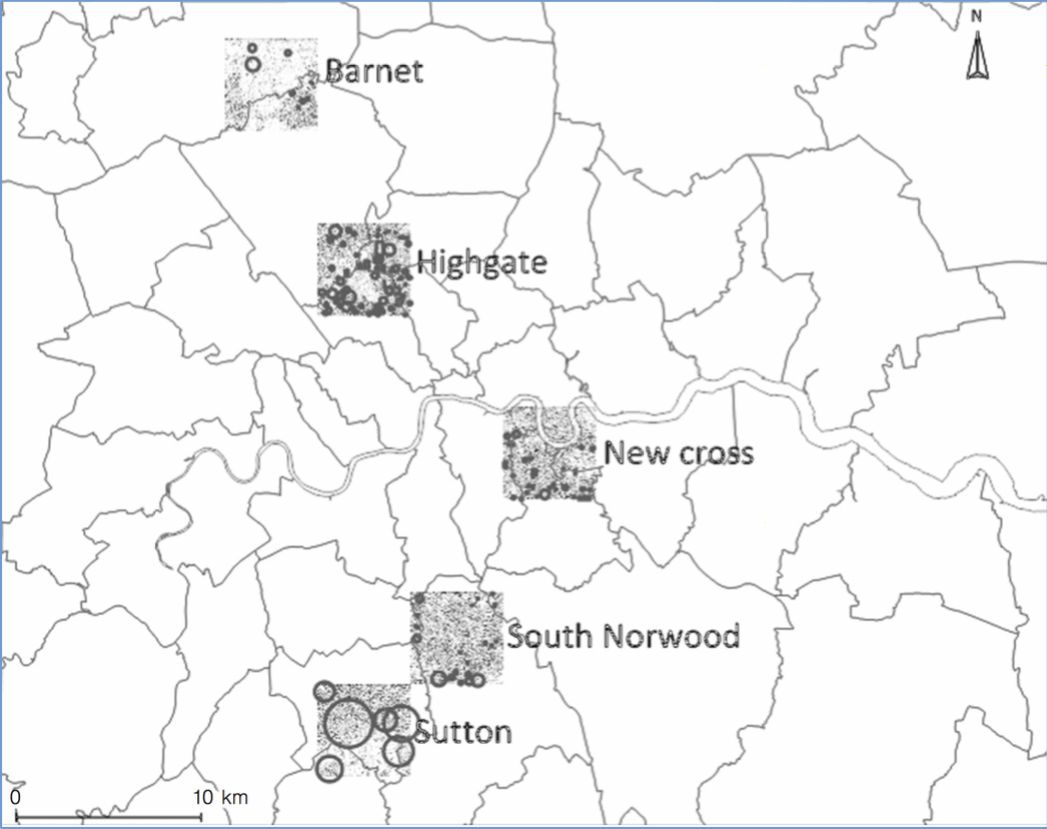
\includegraphics[width=0.95\textwidth]{london-sample-1.png}
    	\caption{This picture should not be here, but apparently it is a nightmare in LaTeX.}
    	\label{fig:london_sample_1}
    \end{figure*}
    
    More precisely, a road is considered in scope if its bounding box, as defined by Ordnance Survey's "Open Names", is completely included in any of the five tiles. 
    
    [SOME WORDING FROM THAT PAPER TO STATE HOW WE DID NOT SIMPLIFY THE PROBLEM BY DOING THIS BUT JUST REDUCED IT IN SIZE].
     
    \textbf{Named vs numbered roads.} Roads that are identified by a number only, e.g. as for motorways, will be considered out of scope.
    
    \textbf{Reliability of the sources.} Only open data from authoritative sources was considered as an option in defining the approach, such as government bodies', and it is assumed to be of the highest possible quality, equivalent to what could be called {\it ground truth}. This allowed the approach not to include any validation of the sources.

\subsection{A social machines mix for OLAF}

    The open data available during our research makes it possible to divide the creation of OLAF in two main sub-problems {\it p1} and {\it p2}. 
    
    \begin{itemize}
        \item {\it p1}: Create a list of all existing {\it house numbers} for each road listed in Ordnance Survey's "Open Names".
        \item {\it p2}: Create a list of all existing {\it house names} for each road listed in Ordnance Survey's "Open Names".
        \item {\it p3}: Create a list of the associations between each of the house number and names above and the list of current\footnote{Postcodes can change. The problem of documenting how addresses change postcode in time is relevant but outside of the scope of research.} postcodes listed in Ordnance Survey's "Open Names". 
    \end{itemize}

    For simplicity, we use the terms "place", "road" and "street" interchangeably, as they are equivalent from a data model perspective in OLAF.

    Open Names "lists definitive place names, roads numbers and postcodes in Great Britain"\footnote{See \url{https://www.ordnancesurvey.co.uk/business-and-government/products/os-open-names.html}.}. It was central to the research work as it is dataset that is functionally closer to the target. OLAF is - in practical terms - equivalent to adding just one dimension to Open Names, that is the list of house names and number for each of its roads. 
    
    Problems {\it p2}\footnote{Note that 98\% of UK addresses are characterised by a house number rather than a house name, so solving {\it p1} is substantially more relevant to achieve completeness in OLAF than {\it p2}.} and {\it p3} are not discussed in this paper. 
    
    Problem {\it p1} can be further decomposed, thanks to the availability of additional open data sources:
    
    \begin{itemize}
        \item {\it p1.1}: Collect the list of house numbers and house names for each existing road as they are referenced in Land Registry's "Price Paid".
        \item {\it p1.2}: Statistically infer the existence of house numbers from the house numbers collected above.
        \item {\it p1.3}: Enable the application of {\it p1.2} through surveying.
        \item {\it p1.4}: Correct the output of {\it p1.2} through surveying.
    \end{itemize}

    \subsubsection{{\it p1.1}: Collect the list of house numbers and house names for each existing road as they are referenced in Land Registry's "Price Paid".} 

        References to existing house names and numbers can be found in a few open data publications in the UK. The largest in size is the "Price Paid Data" by the Land Registry: a non-ministerial Government department with the responsibility to register the ownership of land and property in England and Wales. Data for each ownership transfer since 1995 - and the full address of the building - is available as open data and updated monthly.
        
        20 years of record make an impressive collection of house names and numbers [MORE ABOUT WHAT THE OUTPUT OF THIS IS]

    \subsubsection{{\it p1.2}: Statistically infer the existence of house numbers from the house numbers collected above.} 

        Each culture developed in time a convention for the assignment of house number and names to buildings. In the UK numbering was likely introduced in the early 18th Century as an alternative to house names. Buildings typically are numbered sequentially starting from 1, corresponding to the extremity of the road that is closest to the centre of the town the street is associated to. Odd numbers are on the left-hand side as seen from the centre, even number on the right-hand side. Intermediate properties usually have a number suffixed by one or more letters, this is typical of larger buildings that at some point in time got divided into more smaller dwellings. Modern buildings that have been named by their owner usually retain also a number, that was used by the local government authority during planning.
        
        Centuries of house development and using this system informally of course created many exceptions: e.g. there are buildings for whose house number is zero, places where numbers were assigned consecutively, and house numbers that are simply missing. Simple algorithms, though, have a very high probability to apply the numbering model described above to infer the existence of house numbers from other known house numbers. This is intuitive, as: 
        \begin{itemize}
            \item If we know that one even and one odd house numbers exist in a street, it is likely that all other numbers included within those numbers exist, too (e.g. we can infer 11 and 12 from the existence of 10 and 13)
            \item If we know that two even or odd house numbers exist in a street, it is likely that all other even or odd house numbers included within those numbers exist, too (e.g. we can infer 7 from the existence of 5 and 9, but not 6 and 8, as the right-hand side of the street may not have buildings)
            \item If we know that the same house number in a street is suffixed by two different letters, it is likely that all other letters included within those letters exist, too (e.g. we can infer 14B from the existence of 14A and 14C).
        \end{itemize}
        
        This simple inference is one of the simplest that can be implemented. Other available open data sources enable more complex algorithms, e.g. Ordnance Survey's "Open Maps - Local" [NEED TO CHECK] includes summary shapes for the buildings in each British street, hence enabling the detection of how many buildings are present and suggest how some house numbers may be missing.
        
    \subsubsection{{\it p1.3}: Enable the application of {\it p1.2} through surveying.} 

        It is clear from the description of problem {\it p1.2} that the inference of house numbers is enabled by the availability of two or more couples of house numbers that act as "seeds" and allow the inference rules to trigger one or more times, for each road.
        
        82\% of the streets in scope are referenced in Land Registry's "Price Paid. The house numbers sourced from {\it p1.1} create opportunities for inference for the 74\% of roads, inferring ~113k house numbers from ~111k known house numbers [DO I NEED TO DESCRIBE THE CALCULATIONS SOMEWHERE IN THE PAPER OR I JUST LINK TO THE GITHUB REPOSITORY WITH THE CODE? THE CODE AT THE MOMENT DOES NOT CALCULATE THE STATISTICS BUT JUST RUNS THE INFERENCE, THIS STUFF WAS CALCULATED 'BY HAND'.].  
        
        A substantial number of roads though are not described by sufficient data to trigger inference. Problem {\it 1.3} is about creating the minimum set of data capable of creating the largest sets of inferred house numbers. This means identifying the lowest and highest house numbers for each road for which no house numbers are known\footnote{For simplicity, we did not consider the case where one house number only is known for a street. Those roads are considered as roads with no house numbers.}.

        \begin{figure*}
        	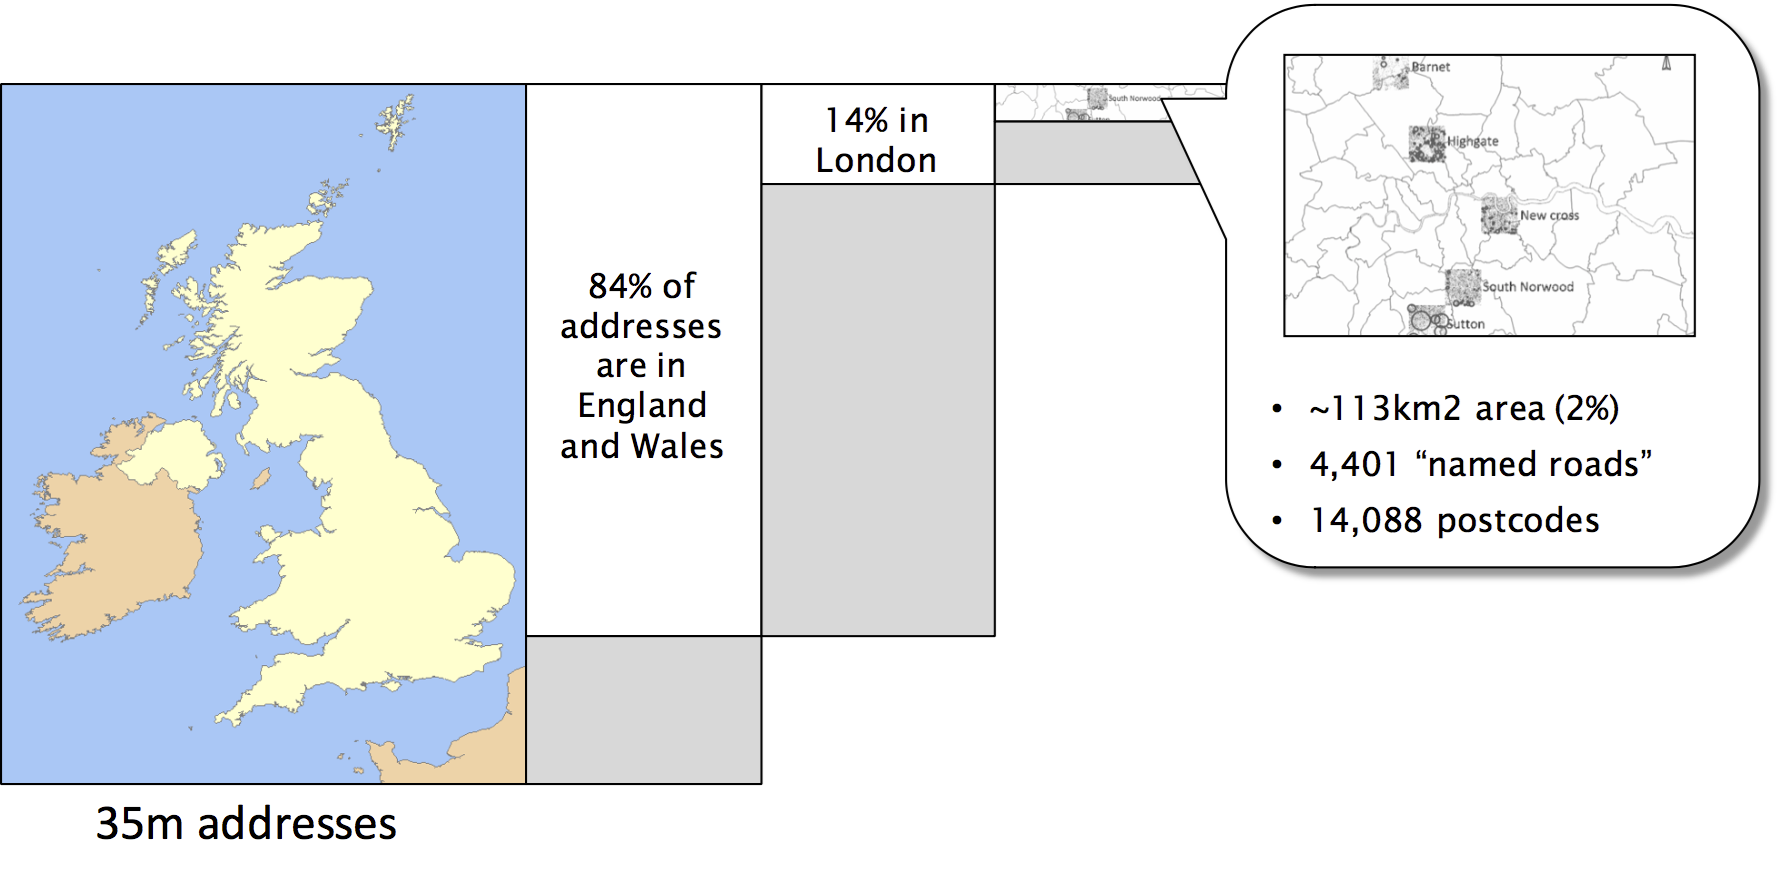
\includegraphics[width=0.95\textwidth]{social-machine-mix-3.png}
        	\caption{This picture should not be here, but apparently it is a nightmare in LaTeX.}
        	\label{fig:social_machine_mix_3}
        \end{figure*}
        
        \begin{figure*}
        	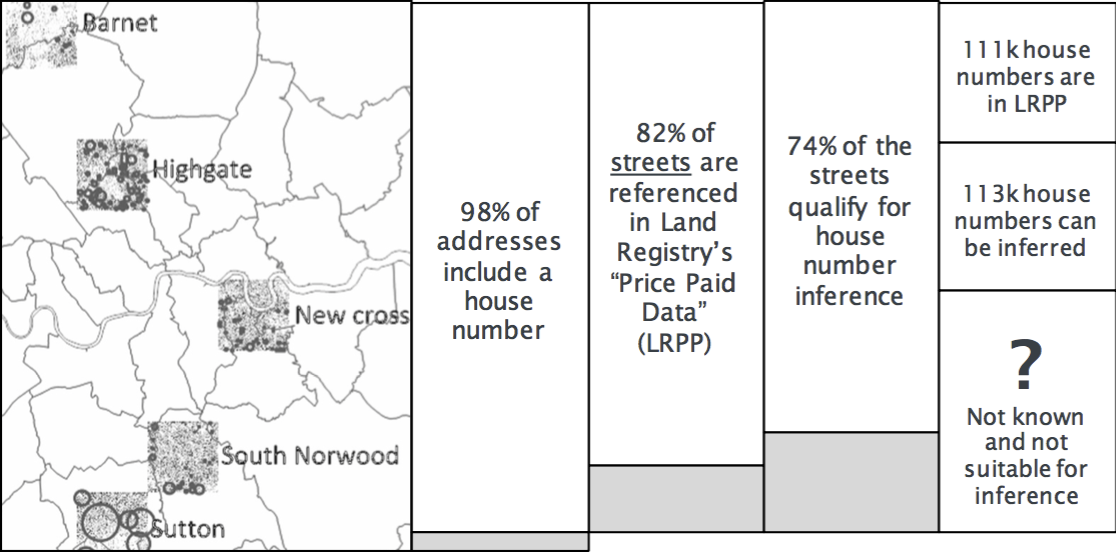
\includegraphics[width=0.95\textwidth]{social-machine-mix-2.png}
        	\caption{This picture should not be here, but apparently it is a nightmare in LaTeX.}
        	\label{fig:social_machine_mix_2}
        \end{figure*}

    \subsubsection{{\it p1.4}: Correct the output of {\it p1.2} through surveying.} 




\subsection{Crowdsourcing house numbers to enable inference}

    \subsubsection{Task model}
    
        The following is a description of the approach that was used for crowdsourcing addresses, that is common to all experimental conditions that were tested.
        
        \textbf{Requester.} The Requester desires to validate the existence of a series of house numbers (e.g. "3" or "7A") in a specified street. Those were previously inferred algorithmically from the observation of \textit{existing} house numbers, as sourced from published open datasets\footnote{See the GitHub repository at \url{https://github.com/Digital-Contraptions-Imaginarium/OLAF-yr2_reference_data} to learn about the reference open data we used, and the repository at \url{https://github.com/Digital-Contraptions-Imaginarium/OLAF-yr2_inference_data} for the inference algorithms.}. When the pictures in the survey tool are of insufficient quality to be read intelligibly (e.g. a house number could be "7A" but it is not clear) it is useful to the Requester to be informed of that. The Requester requires the help of human agents to carry out the tasks, that we will call Workers in the following.
        
        \textbf{Task.} Each HIT (Human Intelligence Task) consists of verifying the existence in a given street of a given specific tuple of inferred house numbers {[}SOME MATHS SYMBOLS HERE{]} that is a subset of the whole set of inferred house numbers for that street {[}SOME MATHS SYMBOLS HERE{]}. 
        
        \textbf{Strategy.} 
        {[}TO BE WRITTEN, DEPENDS ON THE EXPERIMENT SCENARIOS DEFINITION.{]}
        
        \textbf{Crowd $\rightarrow$ Worker.} Each Worker performs her task by declaring, for each house number in the given tuple and street, if a) it can be found by using the survey tool, b) it can't be found or c) it cannot be said with certainty (e.g. if some of the pictures are blurred and could correspond to the house number being searched). Multiple Workers are asked to validate the same tuple and the resulting data is chosen through majority voting.
        
        \textbf{Reliability.} When collecting data to build a dataset that is intended to be published under an open licence, the option to assess its \textit{quality} by comparison with other sources is often not available, for many reason. An alternative source of the same data could simply not be available. Moreover, from an intellectual property perspective, the comparison could make the former "derivative work" of the latter, hence compromising the purpose{[}SOME REFERENCE OR FOOTNOTE TO PUT MORE MEAT AROUND THIS POINT{]}. 
        
        What is possible, instead, is to estimate the \textit{reliability} of the crowdsourced data, independently of any actual knowledge of other sources and/or the ground truth. 
        
        In OLAF's case, the approach described is considered equivalent to what is used for crowdsourcing the acquisition of labels for data items when the labelling is imperfect, that is extensively covered in literature, e.g. in \cite{sheng2008get} or \cite{Welinder:2010vkb}{[STILL HAVE TO READ THE LATTER{]}. 
        
        The quality of the Workers' contribution could be measured by using gold standard tasks \cite{Oleson:2011tx}, e.g. asking them to validate sets of house numbers whose existence is already known. Because of the elementary complexity of the tasks, though, it was assumed that anything standing between the Worker and the actual required tasks would hinder their contribution in volume and quality and compromise furtherance.
        
        Lacking an assessment of the individual Worker's reliability, the option of preferring the best individual Workers vs using multiple labellers becomes unavailable, hence the need to use majority voting. 
        
        For simplicity, all Workers are considered equivalent from a reliability perspective, and the quality of their individual output assumed $ > 0.5 $, so that the \textit{uniform labeller quality} (see \cite{sheng2008get}) of the data chosen through majority voting increases as the number of labellers is increased.
    
    \subsubsection{Recruitment}
    \subsubsection{Design}
    \subsubsection{The virtual survey tool}
    
        Some text before.
        
        \begin{figure*}
        	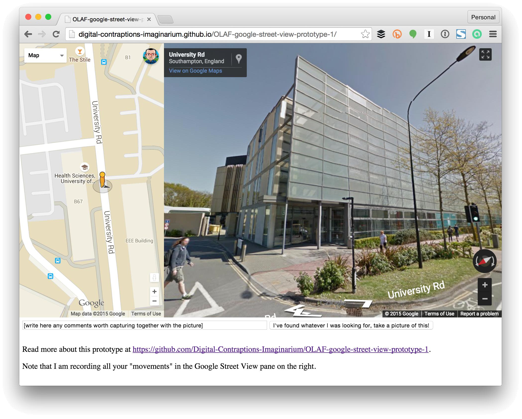
\includegraphics[width=0.95\textwidth]{some_picture.png}
        	\caption{This picture should not be here, but apparently it is a nightmare in LaTeX.}
        	\label{fig:some_figure}
        \end{figure*}
        
        \paragraph{}
        
        Some text after.
        
        [NEEED TO SAY] Unlike other countries, in the UK local authorities do not provide house number plates to the building owners, so this remains their responsibility. Building owners have the option not to affix any plate at all.
    	
    \subsubsection{Scalability}
    
        [THE CALL FOR PAPER EXPLICITLY SAYS THAT "EVIDENCE OF USE IN PRACTICE AND/OR DEMONSTRATION OF SCALABILITY IS REGARDED AS A PLUS"]
    
    \subsubsection{{[}description of additional conditions to test X{]}}
    \subsubsection{{[}description of additional conditions to test Y{]}}

\section{Experiment design}

\subsection{Research hypothesis}
\subsection{Dataset}
\subsection{Evaluation metrics}
\subsection{Experimental conditions}
\section{Results}
% \section{Literature review}
\section{Discussion and conclusion}

{[}The standard EPSRC acknowledgement formula + something about the external reviewers?{]}


\documentclass{article}
\usepackage{url}
\begin{document}
\nocite{*}
\bibliography{main}
\bibliographystyle{splncs03}
\end{document}


\end{document}

